% Created 2021-09-11 Sat 16:40
% Intended LaTeX compiler: xelatex
\documentclass[letterpaper]{article}
\usepackage{graphicx}
\usepackage{grffile}
\usepackage{longtable}
\usepackage{wrapfig}
\usepackage{rotating}
\usepackage[normalem]{ulem}
\usepackage{amsmath}
\usepackage{textcomp}
\usepackage{amssymb}
\usepackage{capt-of}
\usepackage{hyperref}
\usepackage[margin=1in]{geometry}
\usepackage{fontspec}
\usepackage{indentfirst}
\setmainfont[ItalicFont = LiberationSans-Italic, BoldFont = LiberationSans-Bold, BoldItalicFont = LiberationSans-BoldItalic]{LiberationSans}
\newfontfamily\NHLight[ItalicFont = LiberationSansNarrow-Italic, BoldFont       = LiberationSansNarrow-Bold, BoldItalicFont = LiberationSansNarrow-BoldItalic]{LiberationSansNarrow}
\newcommand\textrmlf[1]{{\NHLight#1}}
\newcommand\textitlf[1]{{\NHLight\itshape#1}}
\let\textbflf\textrm
\newcommand\textulf[1]{{\NHLight\bfseries#1}}
\newcommand\textuitlf[1]{{\NHLight\bfseries\itshape#1}}
\usepackage{fancyhdr}
\pagestyle{fancy}
\usepackage{titlesec}
\usepackage{titling}
\makeatletter
\lhead{\textbf{\@title}}
\makeatother
\rhead{\textrmlf{Compiled} \today}
\lfoot{\theauthor\ \textbullet \ \textbf{2021-2022}}
\cfoot{}
\rfoot{\textrmlf{Page} \thepage}
\titleformat{\section} {\Large} {\textrmlf{\thesection} {|}} {0.3em} {\textbf}
\titleformat{\subsection} {\large} {\textrmlf{\thesubsection} {|}} {0.2em} {\textbf}
\titleformat{\subsubsection} {\large} {\textrmlf{\thesubsubsection} {|}} {0.1em} {\textbf}
\setlength{\parskip}{0.45em}
\renewcommand\maketitle{}
\author{Houjun Liu}
\date{\today}
\title{Structure of Cabs, Monomers, Polymers}
\hypersetup{
 pdfauthor={Houjun Liu},
 pdftitle={Structure of Cabs, Monomers, Polymers},
 pdfkeywords={},
 pdfsubject={},
 pdfcreator={Emacs 27.2 (Org mode 9.4.4)}, 
 pdflang={English}}
\begin{document}

\maketitle


\section{Structures of Carbohydrates}
\label{sec:orgeb8c14b}
Each carbohydrate could be a monomer (6 carbons, simple structure). A
carbohydrate monomer (simple sugar) is called a "monosacharide"

\begin{itemize}
\item Two monomers could be chained to build a more complicated structure
named Disachoride
\item Monomers could be chained to build "polymers"
\item Complicated polymers is what forms the energy builds of life
\item The same atoms, with different bonds and hence a different species,
result in "isomers"
\end{itemize}

General chemical formula: \(C_n H_{2n} O\)

\begin{itemize}
\item Monosacharride => a monomer of carbohydrates
\item Disachoride => a dinomer (?) of carbohydrates
\item Polysachride => a polymer of carbohydrates
\end{itemize}

\subsection{Basic Monomers}
\label{sec:orgec2f9a4}
\begin{itemize}
\item Glucose: ring of 6 carbons
\item Fructose: ring of 5 carbons
\end{itemize}

\subsection{The mer-library}
\label{sec:org1eb9610}
\begin{center}
\begin{tabular}{lll}
Name & Note & Composition\\
\hline
Sucrose & Common Sugar & Disachoride: Glucose + Fructose\\
Lactose & The thing that's in milk & Disachoride: Glucose + Galactose\\
Cellose & Plants' cell wall we can't digest & Polysacharides from: beta-Glucose\\
Glucose & Bulding block of sugar & Monomer\\
Galactose & Sugar sweeter than sugar & Monomer\\
Fructose & Controvercial & Monomer\\
Starch & Plant food reserve & Small, branched alpha glucose\\
Glycogen & ANimal energy reserve & Lots of alpha glucose in more branches\\
\end{tabular}
\end{center}

\subsection{Making and Breaking -mers}
\label{sec:orgf406f79}
\textbf{Creating a polymer ("dehydration")}

\begin{itemize}
\item Take monomers
\item Remove water molecules
\item Fill the now-gaping hole with the next monomers
\end{itemize}

\textbf{Breaking a polymer ("rehydration")}

\begin{itemize}
\item Take polymers
\item Add water
\item Get Glucose
\item Profit!
\end{itemize}

Hence, you get thirsty after around 45mins whenever you eat lots of
sugar --- ye gotta get that water to rehydrate and break down those
polymers.

Bonds are called "glycocidic" bonds

\subsection{Alpha vs Beta glucose}
\label{sec:org2b94ebc}
\begin{figure}[htbp]
\centering
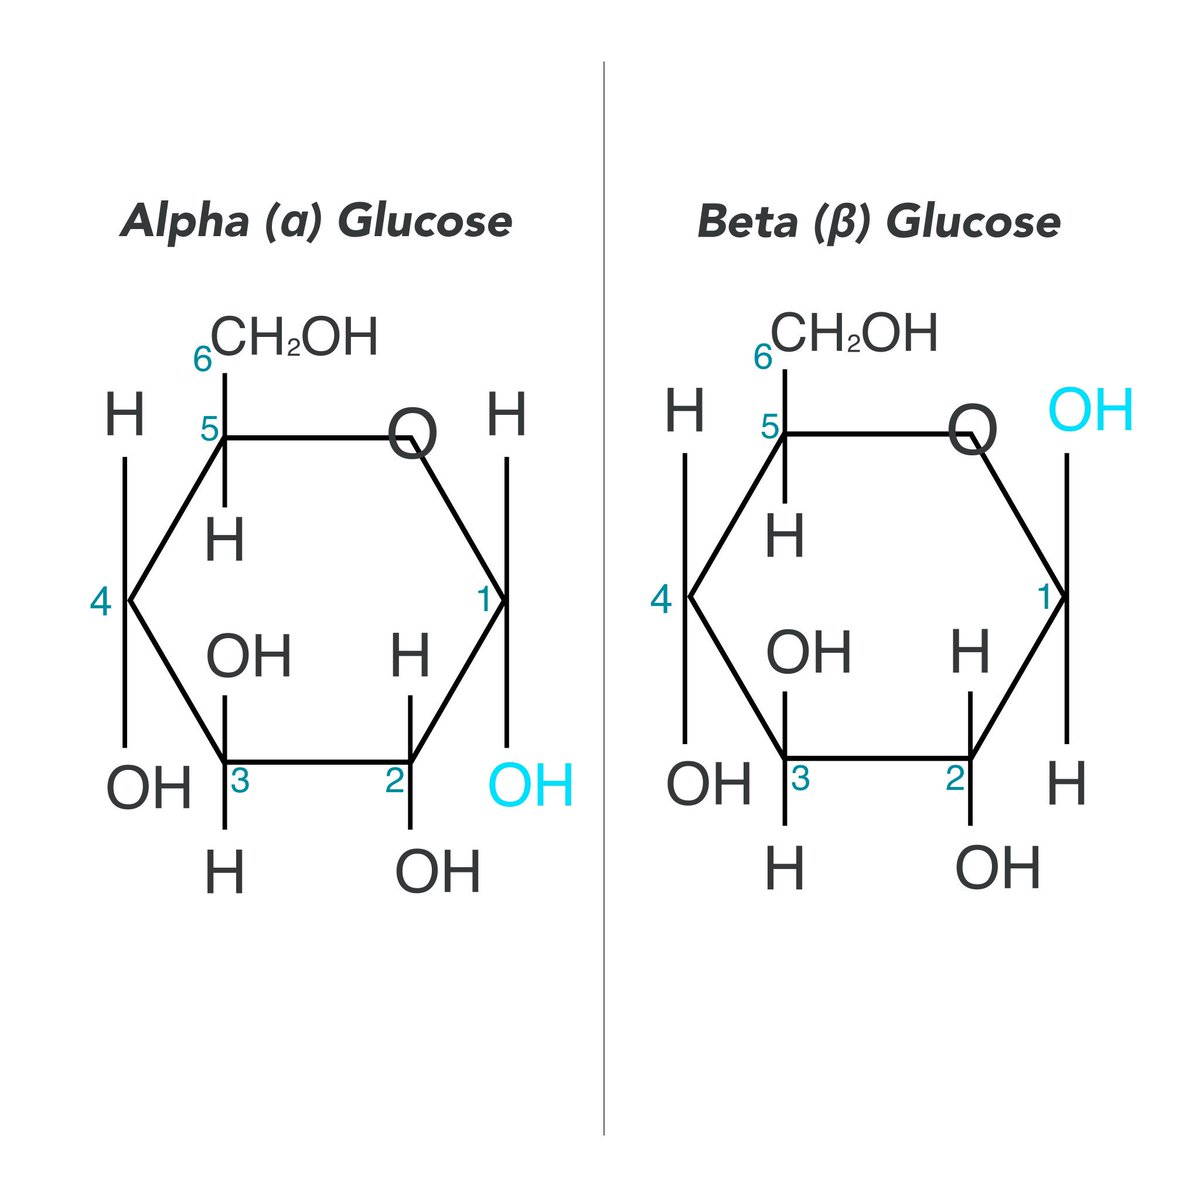
\includegraphics[width=.9\linewidth]{./CrLHc0-WEAAe12C.jpg}
\caption{CrLHc0-WEAAe12C.jpg}
\end{figure}

\noindent\rule{\textwidth}{0.5pt}

And now, a note on energy.

\href{KBhBIO101Enthalpy.org}{KBhBIO101Enthalpy}

\noindent\rule{\textwidth}{0.5pt}

You could add even more monosachrides/disacharides up to get
polysacharides (starch, fiber, glycogen)

\begin{itemize}
\item We get energy for lots of glucose (the alpha variant of which's
polysacharide is starch), but we can't get any from cellulose (whose
polysacratide is fiber)
\item We eat fiber to maintain gut health + poop goodly. Cellulose is
hydrophillic, meaning that fiber makes your guts lubricated.
\item Polysaccharides linked together by \textbf{glycosidic bonds}.
\end{itemize}

NOTE! \textbf{Whichever carbohydrates you are using, you get energy from
breaking its bonds.}
\end{document}
